\documentclass[12pt]{article}

\usepackage{sbc-template}

\usepackage{graphicx,url}
\usepackage{placeins}
\usepackage{float}


\usepackage[brazil]{babel}
\usepackage[utf8]{inputenc}

\usepackage{algorithm}
\usepackage{algpseudocode}

\usepackage{booktabs}
\newcommand{\tra}[1]{\renewcommand{\arraystretch}{#1}}

\sloppy

\title{Reutilização de Software -- Documentação do Trabalho Prático}
%\subtitle{Um Servidor de Jogos para Ensino de Engenharia de Software}

\author{Danilo Ferreira e Silva\inst{1}}


\address{Departamento de Ciência da Computação -- UFMG
  \email{danilofs@dcc.ufmg.br}
}

\begin{document} 

\maketitle



\section{Introdução}

Jogos didáticos são instrumentos de apoio ao ensino utilizados em diversas áreas do conhecimento. Especificamente, na área de Engenharia de Software, podemos citar como exemplos os jogos \emph{Programs And Programmers} \cite{baker2005pnp} e \mbox{\emph{SimulES}} \cite{figueiredo2007simules}. O trabalho proposto na disciplina tem como objetivo projetar e implementar um sistema, empregando as técnicas vistas em aula, que se enquadre no tema de jogos para ensino de Engenharia de Software.
Alinhado a esses objetivos, este documento descreve o projeto e implementação de um servidor de jogos extensível, na forma de uma Linha de Produtos de Software (SPL).
%, com suporte para o jogo \emph{SimulES} e um jogo de perguntas e respostas.

O restante deste documento está organizado da seguinte forma. Na Seção~\ref{sec:requisites}, apresentamos a visão geral do sistema e o conjunto de características da SPL. Na Seção~\ref{sec:design}, apresentamos as principais decisões de projeto, incluindo o cronograma de atividades, as técnicas utilizadas, a arquitetura adotada e padrões de projeto empregados. Finalmente, na Seção~\ref{sec:examples} detalhamos como gerar e executar um produto, usando como exemplo duas configurações de características diferentes.


\section{Sistema Proposto}
\label{sec:requisites}

O sistema projetado, que foi denominado SEGE, é um serviço Web de jogos. O sistema consiste de um núcleo e um ou mais jogos, desenvolvidos como \emph{plug-ins}. No contexto deste trabalho, foram incluídos dois jogos: \emph{SimulES} e um jogo de perguntas e respostas baseado nas aulas virtuais da disciplina (\emph{Quiz}). No entanto, novos jogos podem ser desenvolvidos desde que eles: (i) sejam baseados em turnos e (ii) em cada turno exista um conjunto finito de ações, que possam ser mapeadas em uma string.

Além do serviço, a SPL inclui um cliente simples, baseado em linha de comando, utilizado para testar o produto. Embora uma interface gráfica Web seja desejável, optamos por não incluí-la no escopo do trabalho por questões de prazo.

A Figura~\ref{img:feature-model} apresenta o modelo de características (\emph{feature model}) da SPL. Além disso, a Tabela~\ref{tab:features} descreve de forma sucinta cada característica do modelo. É importante ressaltar que, além do modelo prever a customizar do protudo pela inclusão/exclusão de jogos, cada jogo também apresenta variabilidade. Por exemplo, o banco de perguntas do jogo \emph{Quiz} pode ser customizado para incluir temas como Arquitetura de Software, Idiomas de Programação, Desenvolvimento Orientaçdo a Aspectos, etc.

\begin{figure}[htb]
\centering
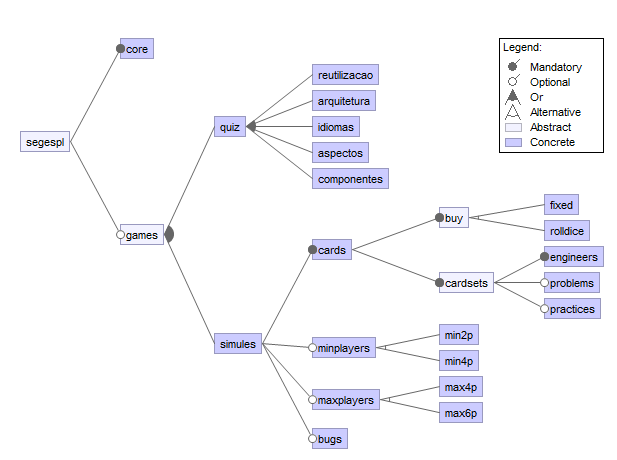
\includegraphics[width=0.8\textwidth]{img/features.png}
\caption{Modelo de características (\emph{feature model})}
\label{img:feature-model}
\end{figure}


\begin{table*}[htb]\centering
\footnotesize
\tra{1.1}
\begin{tabular}{@{}ll@{}}\toprule
\textbf{Característica} & \textbf{Descrição} \\
\midrule
core & Núcleo do sistema, incluindo o serviço Web \\
console\_client & Cliente simples em linha de comando \\
games & Define os jogos disponíveis\\
quiz & Jogo de perguntas e respostas baseado no \emph{quiz} das aulas virtuais\\
questions\_reuse & Conjunto de perguntas de Reutilização de Software\\
questions\_architecture & Conjunto de perguntas de Arquitetura de Software e Padrões Arquiteturais\\
questions\_idioms & Conjunto de perguntas de Idiomas de Programação\\
questions\_aspects & Conjunto de perguntas de Desenvolvimento Orientado a Aspectos\\
questions\_cbse & Conjunto de perguntas de CBSE\\
simules & Jogo SimulES\\
card\_buy\_strategy & Define a estratégia de compra de cartas\\
fixed & Compra um número fixo de cartas por turno\\
rolldice & Compra um número de cartas por turno de acordo com o lançamento de um dado\\
card\_sets & Conjunto de cartas disponíveis\\
engineers & Cartas de engenheiros de software\\
problems & Cartas de problemas\\
practices & Cartas de práticas de Engenharia de Software\\
bugs\_8p & Habilita a existência de bugs\\
min\_players & Habilita a regra de mínimo de jogadores\\
min\_2p & Mínimo de dois jogadores\\
min\_4p & Mínimo de quatro jogadores\\
max\_players & Habilita a regra de máximo de jogadores\\
max\_6p & Máximo de seis jogadores\\
max\_8p & Máximo de oito jogadores\\
\bottomrule
\end{tabular}
\caption{Descrição das características}
\label{tab:features}
\end{table*}


\FloatBarrier
\section{Projeto}
\label{sec:design}

O sistema foi projetado e desenvolvido utilizando uma metodologia semelhanto ao modelo cascata. O planejamento do projeto incluiu cinco atividades principais, descritas na Tabela~\ref{tab:activities}.~\footnote{A implementação do módule SimulES não foi concluída}
%Primeiramente, foi feito um estudo de qual tecnologia seria utilizada para implementar a SPL proposta, priorizando a adoção das técnicas vistas em sala. Em seguida foi construído o modelo de características, identificando os pontos de variabilidade do sistema. O terceiro passo foi a definição da arquitetura do sistema 

\begin{table*}[htb]\centering
\tra{1.1}
\begin{tabular}{@{}lll@{}}\toprule
\textbf{Tarefa} & \textbf{Responsável} & \textbf{Prazo} \\
\midrule
Estudar e escolher tecnologia para suporte a SPL & Danilo & 30/09 \\
Modelagem das características & Danilo & 10/10 \\
Definição da Arquitetura & Danilo & 17/10 \\
Implementação e Testes & Danilo & 14/11 \\
Documentação & Danilo & 14/11 \\
\bottomrule
\end{tabular}
\caption{Cronograma de Atividades}
\label{tab:activities}
\end{table*}


\subsection{Tecnologias Utilizadas}

A SPL foi construída com a ferramenta \textbf{FeatureIDE}~\cite{kastner2009featureide}, utilizando a tecnologia de composição \textbf{FeatureHouse} \cite{apel2009featurehouse}, que dá suporte a Programação Orientada a Características (FOP). %, oferecendo recursos semelhantes aos obtidos com a utilização de \emph{AHEAD}. 
Antes de se chegar a essa decisão, foram considerados também o uso de \emph{AspectJ} e \emph{AHEAD} como mecanismos de composição, mas ambos apresentaram algum inconveniente. No caso da composição com \emph{AspectJ}, a principal dificuldade enfrentada foi que a ferramenta \emph{FeatureIDE} considera que cada característica do modelo está atrelada a um único aspecto. No entanto, esse relacionamento um para um foi considerado inapropriado, visto que uma característica pode ser grande o suficiente para conter diversas classes colaborando entre si para implementá-la.
No caso da composição com \emph{AHEAD}, há suporte apenas para construções Java da versão 1.4. Ou seja, o uso de \emph{generics}, \texttt{enum}, e outras facilidades introduzidas nas versões posteriores não é suportado.

Além das tecnologias de suporte a SPL, foram utilizados também:
\begin{itemize}
\item \textbf{J2EE Servlets}: Padrão J2EE para implementação de aplicações Web.
\item \textbf{Jetty Server}: Servlet Container utilizado.
\item \textbf{JAX-RS}: Padrão J2EE para implementação de serviços REST.
\item \textbf{JBoss RESTEasy}: API que implementa o padrão JAX-RS.
\item \textbf{Google Gson}: API para serialização/deserialização de objetos no formato JSON.
\item \textbf{IvyDE Plug-in}: Plug-in do Eclipse que dá suporte a gestão de dependências de bibliotecas externas via Apache Ivy.
\end{itemize}

\subsection{Arquitetura}

A Figura~\ref{img:architecture} representa a arquitetura do sistema. O sistema utiliza o padrão arquitetural \textbf{cliente--servidor}, cujo elemento principal é o serviço Web \emph{SEGE Core}. Esse serviço expõe expõe um conjunto de operações, usando o estilo arquitetural REST~\cite{fielding2000rest} sob o protocolo HTTP. Dessa forma, há uma flexibilidade para implementar clientes em qualquer tipo de tecnologia, incluindo uma interface Web. Como a tecnologia Web utilizada foi baseada em J2EE, é necessário executar o serviço em um \emph{Servlet Container} (e.g. \emph{Jetty, Apache Tomcat}, etc).

\begin{figure}[htb]
\centering
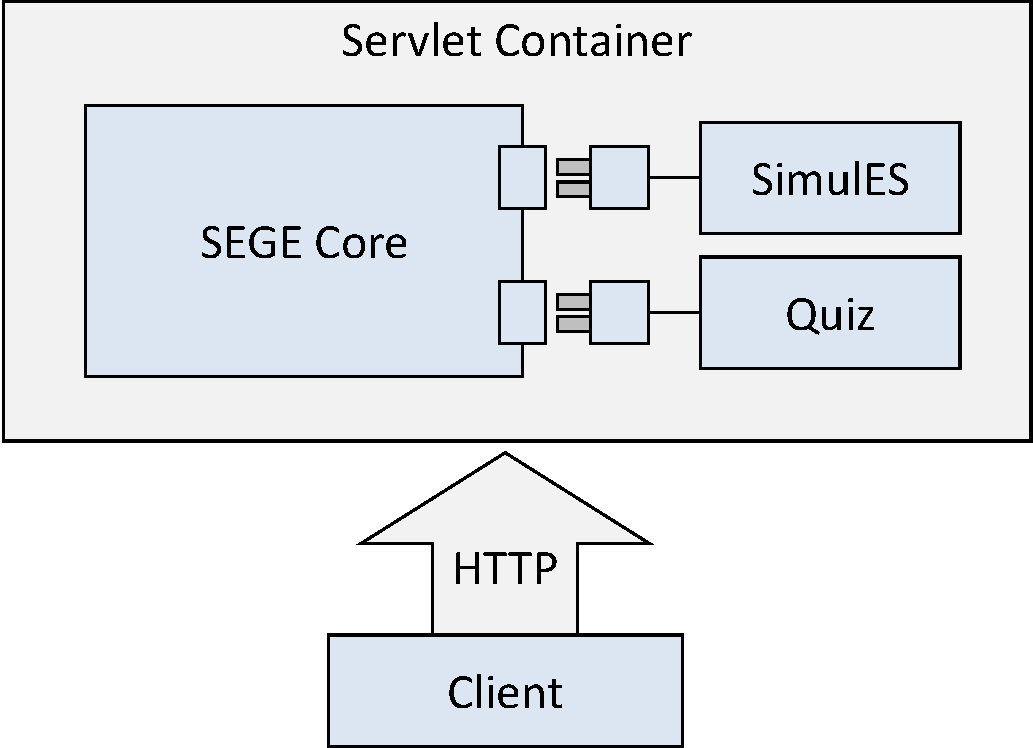
\includegraphics[width=0.5\textwidth]{img/architecture.pdf}
\caption{Arquitetura}
\label{img:architecture}
\end{figure}

Além disso, internamente o serviço utiliza o padrão arquitetural \textbf{microkernel}, onde existe um núcleo mínimo oferecendo um arcabouço geral para implementação dos jogos, mas cada jogo específico é um \emph{plug-in}. Para isso, um jogo deve implementar interfaces básicas exigidas pelo núcleo e deve ser responsável por gerenciar seu estado interno e enumerar as ações disponíveis para os jogadores.

\subsubsection{Interface do Serviço de Jogos}

O serviço de jogos é baseado no estilo arquitetural REST e fornece um conjunto de operações para interagir com o servidor de jogos, conforme listado na Tabela~\ref{tab:operations}. Entre as operações podemos citar: listar as salas, entrar em um jogo, iniciar a partida e postar ações durante a partida. 

\begin{table*}[htb]\centering
\footnotesize
\tra{1.1}
\begin{tabular}{@{}llll@{}}\toprule
\textbf{Verbo HTTP} & \textbf{URL} & \textbf{Parâmetros} & \textbf{Descrição} \\
\midrule
GET & \texttt{games} & & Lista as salas disponíveis \\
GET & \texttt{games/\{gameId\}/\{playerId\}} & & Exibe o estado do jogo \\
PUT & \texttt{games/\{gameId\}/\{playerId\}} & & Adiciona jogador na sala \\
DELETE & \texttt{games/\{gameId\}/\{playerId\}} & & Remove jogador da sala \\
POST & \texttt{games/\{gameId\}/\{playerId\}/start} & & Inicia a partida \\
POST & \texttt{games/\{gameId\}/\{playerId\}/do} & \texttt{\{action\}} & Submete uma ação \\
\bottomrule
\end{tabular}
\caption{Operações do serviço de jogos}
\label{tab:operations}
\end{table*}

Todas as operações do serviço retornam a resposta como um documento no formato \emph{Javascript Object Notation} (JSON). Todas as informações necessárias para representar o estado do jogo sob a perspectiva de um determinado jogador são representadas nesse documento, como exemplificado na Figura~\ref{img:json}. Além disso, por padrão existe sempre uma chave \texttt{actions} que contém a lista das ações específicas do jogo que estão disponíveis para o jogador.

\begin{figure}[htb]
\centering
\footnotesize
\begin{verbatim}
> curl -X GET http://localhost:8080/games/quiz/danilo
{
  "gameId": "quiz",
  "status": "started",
  "state": {
    "score": {
      "danilo": 1
    },
    "currentRound": 4,
    "currentPlayer": "danilo",
    "question": "As seguintes opções são potenciais problemas associados a
                 reutilização de software, exceto.",
    "options": {
      "1": "Falta de ferramentas de suporte",
      "2": "Manutenção de uma biblioteca de componentes",
      "3": "Maiores custos de manutenção",
      "4": "Maior treinamento da equipe"
    }
  },
  "actions": ["1", "2", "3", "4"]
}
\end{verbatim}
\caption{Exemplo de requisição e resposta em JSON, representando o estado do jogo e ações disponíveis}
\label{img:json}
\end{figure}

\subsubsection{Plug-ins de Jogos}

Jogos são adicionados ao servidor na forma de plug-ins. Para tal, é necessário implementar a interface \texttt{GamePlugin} para o jogo em questão. Além disso, o jogo deve ser registrado no arquivo de configuração \texttt{games.xml}, indicando um identificador do jogo e o nome qualificado da classe que o implementa. A Figura~\ref{img:gamesxml} mostra um exemplo de tal arquivo.

\begin{figure}[htb]
\centering
\footnotesize
\begin{verbatim}
<?xml version="1.0" encoding="UTF-8" standalone="no"?>
<games>
  <game id="simules" gameClass="sege.simules.SimulEs"/>
</games>
\end{verbatim}
\caption{Exemplo de configuração do arquivo \texttt{games.xml}}
\label{img:gamesxml}
\end{figure}

É interessante ressaltar que a composição com \emph{FeatureHouse} é capaz de tratar arquivos XML, fazendo a combinação de seus nodos em um único arquivo. Isso permite que a configuração, assim como o código, fique modularizado dentro do diretório da característica.

\subsection{Padrões de Projeto}

Os seguintes padrões de projeto foram utilizados na implementação do código:
\begin{itemize}
\item \textbf{Facade}: A interface interface \texttt{GameService} funciona como uma fachada para o servidor de jogos.
\item \textbf{Adapter}: A classe \texttt{RestGameService} adapta a interface \texttt{GameService}, delegando as chamadas de métodos mas modificando o tipo de retorno para uma resposta HTTP.
\item \textbf{Abstract Factory}: A interface \texttt{GamePlugin} funciona como uma fábrica abstrata, pois apenas uma implementação específica de um jogo conhece qual tipo de objeto deve ser criado pelo método \texttt{createInitialState} para representar o estado interno.
\item \textbf{State}: A classe \texttt{GameRoom}, que representa uma instância de um jogo em execução, utiliza um objeto do tipo \texttt{InternalGameState} para representar o estado interno de um jogo e delega a responsabilidade de obter e aplicar as ações disponíveis para esse objeto.
\item \textbf{Command}: A classe \texttt{ConsoleClient} lê uma linha do console e a trassforma em um objeto que representa om comando, para que ele possa ser invocado posteriormente de forma centralizada.
\end{itemize}

\section{Instruções de Uso e Exemplos}
\label{sec:examples}

\subsection{Configuração e compilação de produtos}

O pacote distribuído contém o código fonte organizado como um projeto Eclipse. Para importar tal projeto, é necessário ter instalado no Eclipse os plug-ins \emph{FeatureIDE} (com o módulo \emph{FeatureHouse}) e \emph{IvyDE}. Os passos para configuração e compilação de um produto são:
\begin{itemize}
\item Importar o projeto no \emph{workspace}.
\item Acionar o comando \emph{Resolve all} do \emph{IvyDE} para recuperar as depedências para arquivos JAR de API's externas.
\item Criar ou modificar uma configuração existente na pasta \texttt{configs} e selecioná-la como configuração corrente.
\item Executar a classe \texttt{WebServer} como aplicação Java para iniciar o servidor. Alternativamente, pode ser usada a classe \texttt{ConsoleClient} para testar a aplicação mais facilmente, pois ela já roda cliente e servidor em um único processo e oferece uma interface em linha de comando para interação.
\end{itemize}

\subsection{Exemplos de produtos}

O sistema contém duas configurações de produtos, para fins de exemplo:
\begin{itemize}
\item \textbf{product1} Servidor com o jogo Quiz, com perguntas sobre Desenvolvimento Orientado a Aspectos e Engenharia de Software Baseada em Componentes.
\item \textbf{product2} Servidor com o SimulES, com um mínimo de 2 jogadores, sem incluir cartas de práticas de ES.
\end{itemize}

\FloatBarrier
\bibliographystyle{sbc}
\bibliography{bibfile}

\end{document}
